% Autor: Alfredo Sánchez Alberca (email:asalber@ceu.es)
% Charts that shows the purpose of Statistics
\begin{tikzpicture}[every label/.style={text=color1}]
\tikzstyle{node} = [align=center, node distance=1cm, text=color1]; 
\tikzstyle{arrow} = [-latex, color2, line width=10pt];

\node (data) [label=-90:Data] at (0,1) {\includegraphics[height=1.5cm]{img/introduction/data.pdf}}; 
\pause
\node (information) [label=-90:Information] at (4,1) {
\includegraphics[height=1.5cm]{img/introduction/information.png}};
\draw[arrow] (data) -- (information) node[midway,white,font=\footnotesize] {STATISTICS\quad\phantom{0}};
\pause
\node (knowledge) [label=-90:Knowledge] at (8,1) {\includegraphics[height=1.5cm]{img/introduction/knowledge.png}};
\draw [arrow] (information) -- (knowledge) node[midway,white,font=\footnotesize] {Interpretation\quad\phantom{0}};
\pause
\node (decisions) at (11,1) {\phantom{0}};
\draw [arrow] (knowledge) -- (decisions) node[midway,white,font=\footnotesize] {Decisions\quad\phantom{0}};
\end{tikzpicture} 